\chapter{Agenda tříd}
\section{Popis problému}
Implementace agendy tříd v rozvrhovém API školního systému představuje komplexní úkol, jehož řešení vyžaduje pečlivé zvážení a hluboké pochopení jak administrativních aspektů pro správu školy, tak technických. Tento problém je esenciální pro správné fungování školního systému, který musí být schopen efektivně spravovat nejen aktuální rozvrhy a třídy, ale také uchovávat historická data.

\section{Úvod do problematiky}
Školní rozvrhový systém je srdcem administrativy školy, zajišťující, že učitelé, žáci a učebny jsou správně přiděleni v rámci různých časových bloků během školního roku. Tento systém musí zvládat nejen plánování aktuálních rozvrhů, ale také uchovávání historických dat.

\section{Požadavky}
Pro lepší pochopení problému je důležité nahlédnout do širších souvislostí. Školní systém musí splňovat následující požadavky:

\begin{itemize}
    \item \textbf{Konzistence dat:} Zajištění, že data o třídách, rozvrzích a žácích jsou konzistentní napříč různými časovými obdobími.
    \item \textbf{Historická data:} Uchovávání historických záznamů pro administrativní účely.
    \item \textbf{Flexibilita:} Systém musí být schopen flexibilně reagovat na změny, jako je přechod žáků mezi třídami, změny učitelů a učeben.
\end{itemize}

V kontextu školního rozvrhového systému se agenda tříd týká správy informací o třídách, které zahrnují aktuální třídy, jejich žáky, rozvrhy, záznamy probrané látky (\ref{sec:lesson-evidence} třídnice) a absence. Systém musí být schopen všechny změny správně zaznamenat a reflektovat. Zmíněný úkol je komplikován několika faktory:

\begin{enumerate}
    \item \textbf{Horizontální přechody studentů:} Žák během studia v průběhu školního roku může změnit třídu, obor nebo třeba školu za speficických podmínek, který stanovuje školský zákon a ředitel školy.
    \item \textbf{Vertikální přechody studentů:} Žák, který nesplní zákonné požadavky pro postup do dalšího ročníku, tedy neprospěl, může být zařazen v následujícím školním roce do jiné třídy a ročník opakovat. Žák též může vzdělávání přerušit, či školu opustit.
    \item \textbf{Přerušení studia:} Student může během probíhajícího studia požádat ředitele školy o přerušení vzdělávání. Maximální doba trvání přerušení dle zákona § 66 odst. 5 zákona č. 561/2004 Sb. školský zákon - znění od 01.01.2024 \cite{skolsky-zakon-preruseni-obyc} až na dobu dvou let s výjimkou mateřství \cite{skolsky-zakon-preruseni-materstvi}, které se řídí jiným procesem.
    \item \textbf{Administrativní a kontrolní požadavky:} Uchovávání dat pro administrativní, právní a legislativní důvody, kterým mohou být inspekce státními orgány nebo například soudy.
\end{enumerate}

Z těchto důvodů je implementace agendy tříd ve školním rozvrhovém systému složitá a vyžaduje pečlivé zvážení různých přístupů. Je důležité navrhnout systém, který bude nejen efektivní a flexibilní, ale také bude splňovat všechny uvedené požadavky. V následujících částech této kapitoly se budeme podrobněji zabývat jednotlivými návrhy implementace a jejich dopady na celkovou konzistenci a funkčnost školního systému.

\section{Návrhy implementace}
Na základě výše uvedených požadavků a kontextu jsou navrženy tři hlavní přístupy k implementaci agendy tříd v rozvrhovém API:

\begin{enumerate}
    \item \textbf{Ukládání pouze aktuálního ročníku a aktuálních rozvrhů:} Tento přístup minimalizuje datovou zátěž na serveru tím, že uchovává pouze informace o aktuálním ročníku a rozvrzích. Historická data jsou uložena na odděleném administrativním serveru.

    \begin{figure}[H]
        \centering
        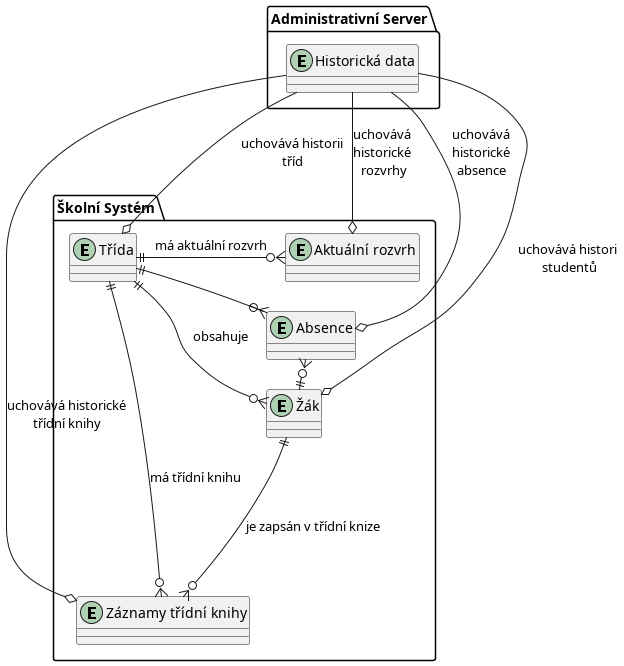
\includegraphics[width=\textwidth]{ed-schedule-only-actual.png}
        \caption{Ukládání pouze aktuálního ročníku a aktuálních rozvrhů}
        \label{fig:ed-schedule-only-actual}
    \end{figure}
    
    Před začátkem každého školního roku by bylo tedy potřeba sjednat synchronizační proces pro archivování dat na administrativní server, smazání z rozvrhového serveru a nahrání nových dat. Tento synchronizačí mechanismus by mohl být obtížný pro správný chod. Předpokládáme, že oba servery spravuje jiný zaměstnanec. V případě chyby v programu způsobené programátory by bylo možné nenávratně přijít o důležitá data.

    \item \textbf{Třída definována prefixem, suffixem, datem vytvoření a kalkulovaným ročníkem:} Tento přístup ukládá informace o třídách pomocí kombinace prefixu, suffixu a data vytvoření třídy. Ročník je kalkulován jako rozdíl mezi datem vytvoření a začátkem aktuálního školního roku.

    \begin{figure}[H]
        \centering
        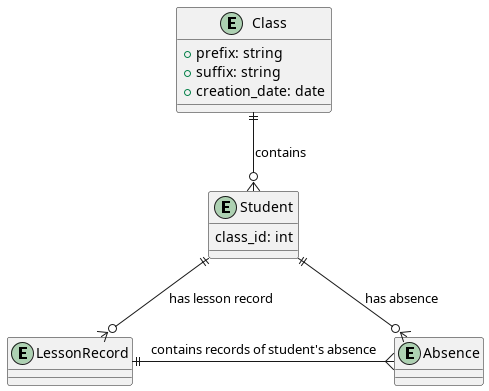
\includegraphics[width=0.6\textwidth]{ed-schedule-calculated-class.png}
        \caption{Relační schéma varianty s kalkulovaným ročníkem}
        \label{fig:ed-schedule-only-actual}
    \end{figure}

    \begin{figure}[H]
        \centering
        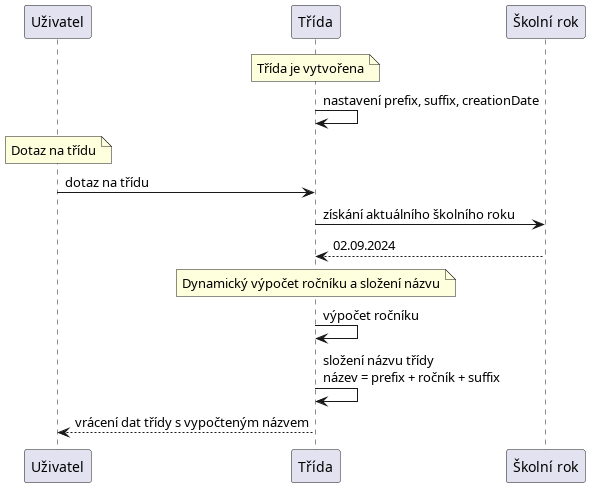
\includegraphics[width=\textwidth]{td-schedule-calculated-class.png}
        \caption{Schéma průběhu dotazu na jméno třídy}
        \label{fig:td-schedule-calculated-class}
    \end{figure}
    
    Problémem v tomto případě je samotná kalkulace. Pro dodržení aktuálnosti dat, musí být ročník vždy vypočítán, protože jakákoliv forma uchovávání mezivýsledku by mohla vést k nekonzistenci v čase. Pokud dorazí požadavek k získání aktuálních tříd, musí server vypočíst všechny ročníky a spojit celé jméno třídy.

    Dalším problémem tohoto řešení jsou propadlí nebo přecházející žáci. Jakmile žák propadne, nastávají 2 varianty řešení:
    \begin{itemize}
        \item odebrat žáka z aktuální třídy a přiřadit jej do nové třídy, ale ztratí minulé záznamy, protože třída je jedním z atributů žáka.

        Řešením může být např. psané záznamy o změnách, avšak nepokryjí všechny požadavky pro snadnou manipulaci s daty.
        \item vytvoření nového žáka, který začíná studovat v pokročilém ročníku. Tím by byla zajištěna konzistence dat, avšak duplicitní účty pro jednoho žáka.

        Řešením může být propojení minulých účtů žáka s novými (relací 1:N), kde žák by měl uložené své minulé účty. Stále je problém, že to není řešení příčiny, ale důsledku.
        \begin{figure}[H]
            \centering
            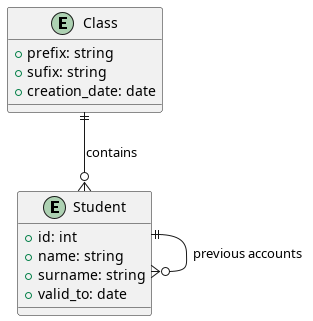
\includegraphics[width=0.5\textwidth]{ed-schedule-calculated-previous-relation.png}
            \caption{Schéma vazby na předchozí účty}
            \label{fig:ed-schedule-calculated-previous-relation}
        \end{figure}
    \end{itemize}

    \item \textbf{Třída definována celým názvem a datem validity od - do:} Tento přístup zahrnuje kompletní informace o třídě včetně ročníku a platnosti od-do. Každý rok se vytváří nové třídy a vztahy mezi studenty a třídami jsou zaznamenány pomocí M:N tabulky.

    \begin{figure}[H]
        \centering
        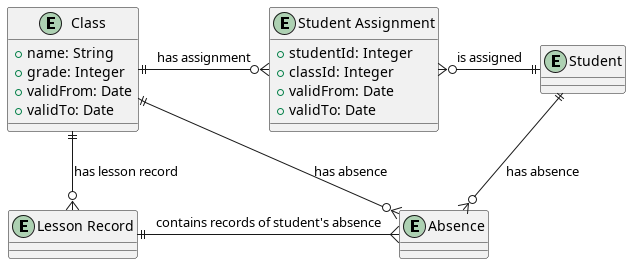
\includegraphics[width=0.9\textwidth]{ed-schedule-validity-from-to.png}
        \caption{Schéma vazby M:N pro přiřazení třídy v návrhu od - do}
        \label{fig:ed-schedule-validity-from-to}
    \end{figure}

    \begin{figure}[H]
        \centering
        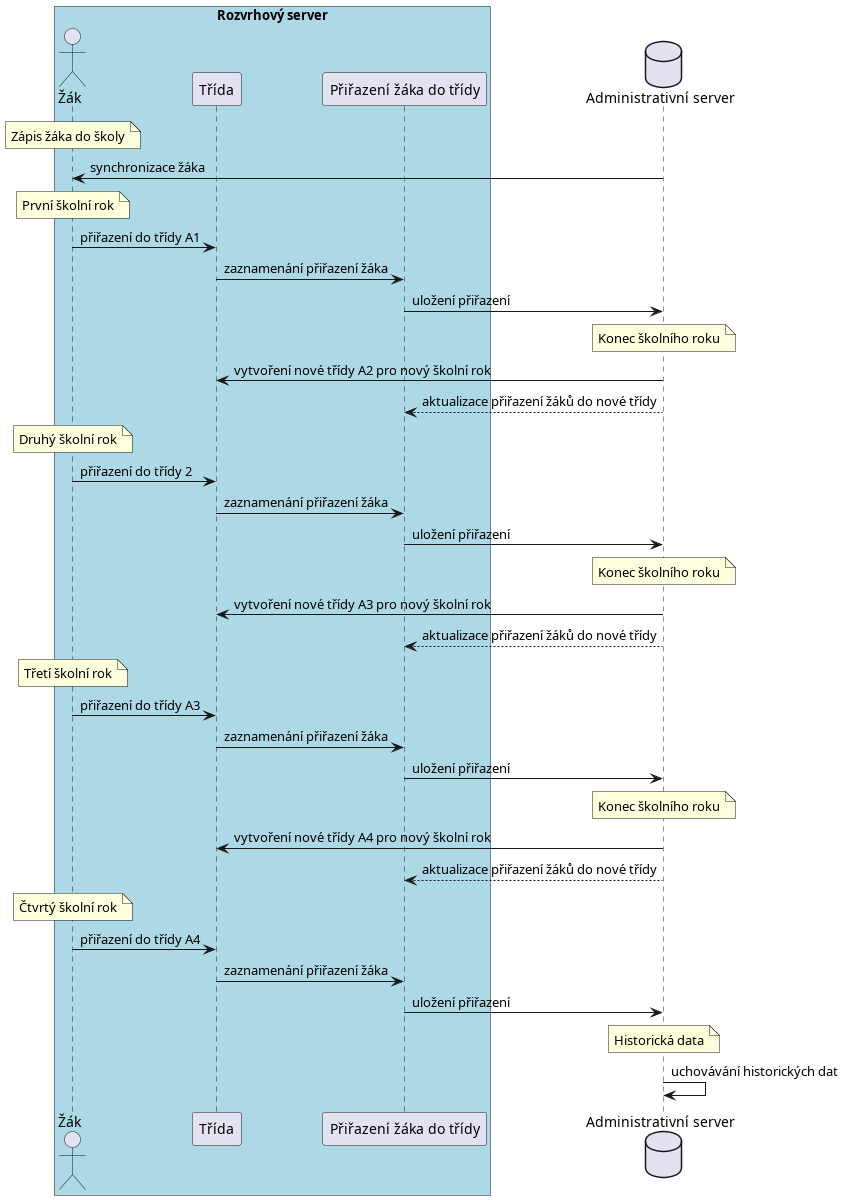
\includegraphics[width=\textwidth]{td-schedule-validity-from-to.png}
        \caption{Schéma průchodu žáka školním procesem z podlehu rozvrhů v návrhu validity od - do}
        \label{fig:td-schedule-validity-from-to}
    \end{figure}
    
    Hlavní výhodou tohoto řešení je konzistence dat i při přesunu žáků v třídách. V tom případě stačí ukončit validitu dotčených tříd, vytvořit nové se stejným názvem a přiřazení nových žáků ve správném pořadí.

    Nevýhodou je vyšší náročnost dotazování na třídu konkrétního žáka. Databáze musí projít všechny přiřazené třídy žáka, vybrat tu aktuálně validní dle dat validity a následně třídu vybrat.

\end{enumerate}

